\documentclass[pdf]{beamer}
\mode<presentation>{
    \usetheme{Warsaw}
    \usecolortheme{seahorse} % Adds a gentle color theme
    \setbeamertemplate{navigation symbols}{} % Remove navigation symbols
    \setbeamertemplate{footline}[frame number] % Add slide numbers
}

%% preamble
\title{CUR Decomposition and Its Applications}
\subtitle{A Comprehensive Overview}
\author{Kevin Smith}
\date{\today}

\usepackage{amsmath} % Enhanced mathematics
\usepackage{amsfonts} % Additional fonts
\usepackage{amssymb} % Additional symbols

\begin{document}

\begin{frame}
    \titlepage
\end{frame}

\begin{frame}{Introduction}
    \begin{itemize}
        \item \textbf{Overview of Matrix Factorizations:}
            \begin{itemize}
                \item Matrix factorizations are pivotal in numerical analysis, data science, and signal processing.
                \item Key types: LU, QR, SVD—each serves specific applications and offers different insights into matrix structures.
            \end{itemize}
        \item \textbf{Introduction to CUR Decomposition:}
            \begin{itemize}
                \item CUR selectively uses actual columns and rows from the matrix to form low-rank approximations.
                \item Emphasizes interpretability and efficiency in large, sparse datasets.
            \end{itemize}
    \end{itemize}
\end{frame}

\begin{frame}{Theoretical Background}
    \begin{itemize}
        \item \textbf{Mathematical Definition of CUR:}
            \begin{itemize}
                \item For a given matrix \( A \), CUR decomposition finds matrices \( C \), \( U \), and \( R \) such that \( A \approx CUR \).
                \item \( C \) and \( R \) consist of selected columns and rows from \( A \), while \( U \) is a smaller connecting matrix.
            \end{itemize}
        \item \textbf{Importance in Data Science:}
            \begin{itemize}
                \item Provides an interpretable low-rank approximation useful in scenarios like recommender systems and principal component analysis where interpretability is as crucial as dimensionality reduction.
            \end{itemize}
    \end{itemize}
\end{frame}

\begin{frame}{Mathematical Foundations of Leverage Scores}
    \begin{itemize}
        \item \textbf{Definition and Calculation:}
            \begin{itemize}
                \item Leverage scores quantify the influence of specific rows or columns on the rank-k approximation of \( A \).
                \item Computed as the squared Euclidean norm of the rows of \( V \) in the SVD \( A = U \Sigma V^T \).
            \end{itemize}
        \item \textbf{Role in CUR Decomposition:}
            \begin{itemize}
                \item Guide the selection of columns/rows that best capture the underlying structure of \( A \).
                \item High leverage scores correlate with high influence on the matrix's spectral properties.
            \end{itemize}
        \item \textbf{Statistical Interpretation:}
            \begin{itemize}
                \item Leverage scores can be normalized to sum to one, forming a probability distribution over the columns or rows.
                \item This probabilistic interpretation is crucial for sampling methods in CUR decomposition, emphasizing columns or rows that have a disproportionately large impact on the data structure.
            \end{itemize}
    \end{itemize}
\end{frame}
 

\begin{frame}{Derivation of Leverage Scores}
    \begin{itemize}
        \item \textbf{Definition:} Leverage scores indicate the importance of rows or columns in capturing the data structure.
        \item \textbf{Mathematical Basis:}
            \begin{itemize}
                \item Consider matrix \( A \) of size \( m \times n \) with Singular Value Decomposition (SVD): \( A = U \Sigma V^T \).
                \item The leverage score of the \( i \)-th row of \( U \) (or \( i \)-th column of \( V^T \)) is defined as:
                \[
                l_i = \| U[i,:] \|^2 = U[i,:] \cdot U[i,:]^T
                \]
                \item This represents the squared norm of the \( i \)-th row of \( U \), indicating its contribution to the rank-k approximation.
            \end{itemize}
        \item \textbf{Significance:}
            \begin{itemize}
                \item High leverage scores identify rows/columns that have significant impact on the matrix's spectral properties.
                \item Essential for selecting informative rows/columns in CUR decomposition.
            \end{itemize}
    \end{itemize}
\end{frame}


\begin{frame}{CUR Decomposition Algorithm}
    \begin{block}{Detailed Algorithm}
        \begin{enumerate}
            \item Compute an approximate SVD of \( A \) to obtain \( V \).
            \item Calculate leverage scores for all columns.
            \item Select columns and rows with the highest scores.
            \item Construct \( U \) to minimize \( \| A - CUR \|_F \), typically using the Moore-Penrose pseudoinverse.
        \end{enumerate}
    \end{block}
    \begin{itemize}
        \item \textbf{Computational Considerations:} Efficiency depends on the method for computing or approximating SVD and the sparsity of the matrix.
    \end{itemize}
\end{frame}

\begin{frame}{Spectral Properties and CUR Decomposition}
    \begin{itemize}
        \item \textbf{Impact on Eigenvalues:}
            \begin{itemize}
                \item CUR decomposition approximates the original matrix \( A \) by selecting a subset of its rows and columns.
                \item This selection can alter the spectral properties (eigenvalues) of \( A \), especially if the selected columns/rows are not representative of the entire data.
            \end{itemize}
        \item \textbf{Matrix Conditioning:}
            \begin{itemize}
                \item The conditioning of the matrix \( C \) and \( R \) in CUR can significantly affect the stability and accuracy of the decomposition.
                \item Poorly chosen subsets can lead to a high condition number, which increases the sensitivity to numerical errors.
            \end{itemize}
        \item \textbf{Improving Stability:}
            \begin{itemize}
                \item Using regularization techniques or improved selection algorithms that consider both leverage scores and conditioning can enhance stability.
            \end{itemize}
    \end{itemize}
\end{frame}

\begin{frame}{CUR Decomposition Results}
    \frametitle{Matrix C, U, R and CUR Approximation}
    Matrix \( C \) (Selected Columns based on Leverage Scores):
    \[
    C = \begin{bmatrix} 2 & 1 & 5 \\ 4 & 5 & 1 \\ 3 & 2 & 6 \\ 5 & 6 & 2 \\ 3 & 5 & 4 \end{bmatrix}
    \]
    Matrix \( U \) (Connection Matrix):
    \[
    U = \begin{bmatrix} 0.5 & 0.35714286 & -0.57142857 \\ -0.16666667 & -0.30952381 & 0.42857143 \\ -0.16666667 & 0.11904762 & 0.14285714 \end{bmatrix}
    \]
    Matrix \( R \) (Selected Rows based on Leverage Scores):
    \[
    R = \begin{bmatrix} 5 & 4 & 3 & 2 & 1 \\ 1 & 2 & 3 & 4 & 5 \\ 5 & 3 & 1 & 6 & 4 \end{bmatrix}
    \]
\end{frame}

\begin{frame}{CUR Approximation of Matrix \( A \)}
    \[
    A \approx CUR = \begin{bmatrix} 1 & 2 & 3 & 4 & 5 \\ 5 & 4 & 3 & 2 & 1 \\ 2 & 3 & 4 & 5 & 6 \\ 6 & 5 & 4 & 3 & 2 \\ 5 & 3 & 1 & 6 & 4 \end{bmatrix}
    \]

    \textbf{Leverage Scores Calculation:}
    The leverage score of row \( i \) is calculated using the squared Euclidean norm of the corresponding row in matrix \( V \) from the SVD of \( A \).
    \[
    \text{Leverage Score of Row } i = \| V[i, :] \|^2 = \sum_{j=1}^{n} V[i, j]^2
    \]
    where \( n \) is the number of columns in \( V \). 
    \[
    LVG Scores: [0.2, 0.2, 0.2, 0.2, 0.2]
    \]
    \textbf{Note:} Each column was equally likely to be selected due to uniform leverage scores.
\end{frame}

\begin{frame}{Statistical and Practical Implications}
    \begin{itemize}
        \item \textbf{Error Analysis:}
            \begin{itemize}
                \item The error of CUR, \( \| A - CUR \|_F \), depends on the quality of column and row selection.
                \item Theoretically, CUR aims to approach the optimal rank-k SVD approximation error.
            \end{itemize}
        \item \textbf{Stability and Robustness:}
            \begin{itemize}
                \item Stability concerns arise from the conditioning of \( C \) and \( R \).
                \item Techniques like regularization or enhanced selection criteria (beyond leverage scores) can mitigate numerical instabilities.
            \end{itemize}
    \end{itemize}
\end{frame}

\begin{frame}{Image Compression with CUR: Original vs. Compressed}
    \begin{figure}
        \centering
        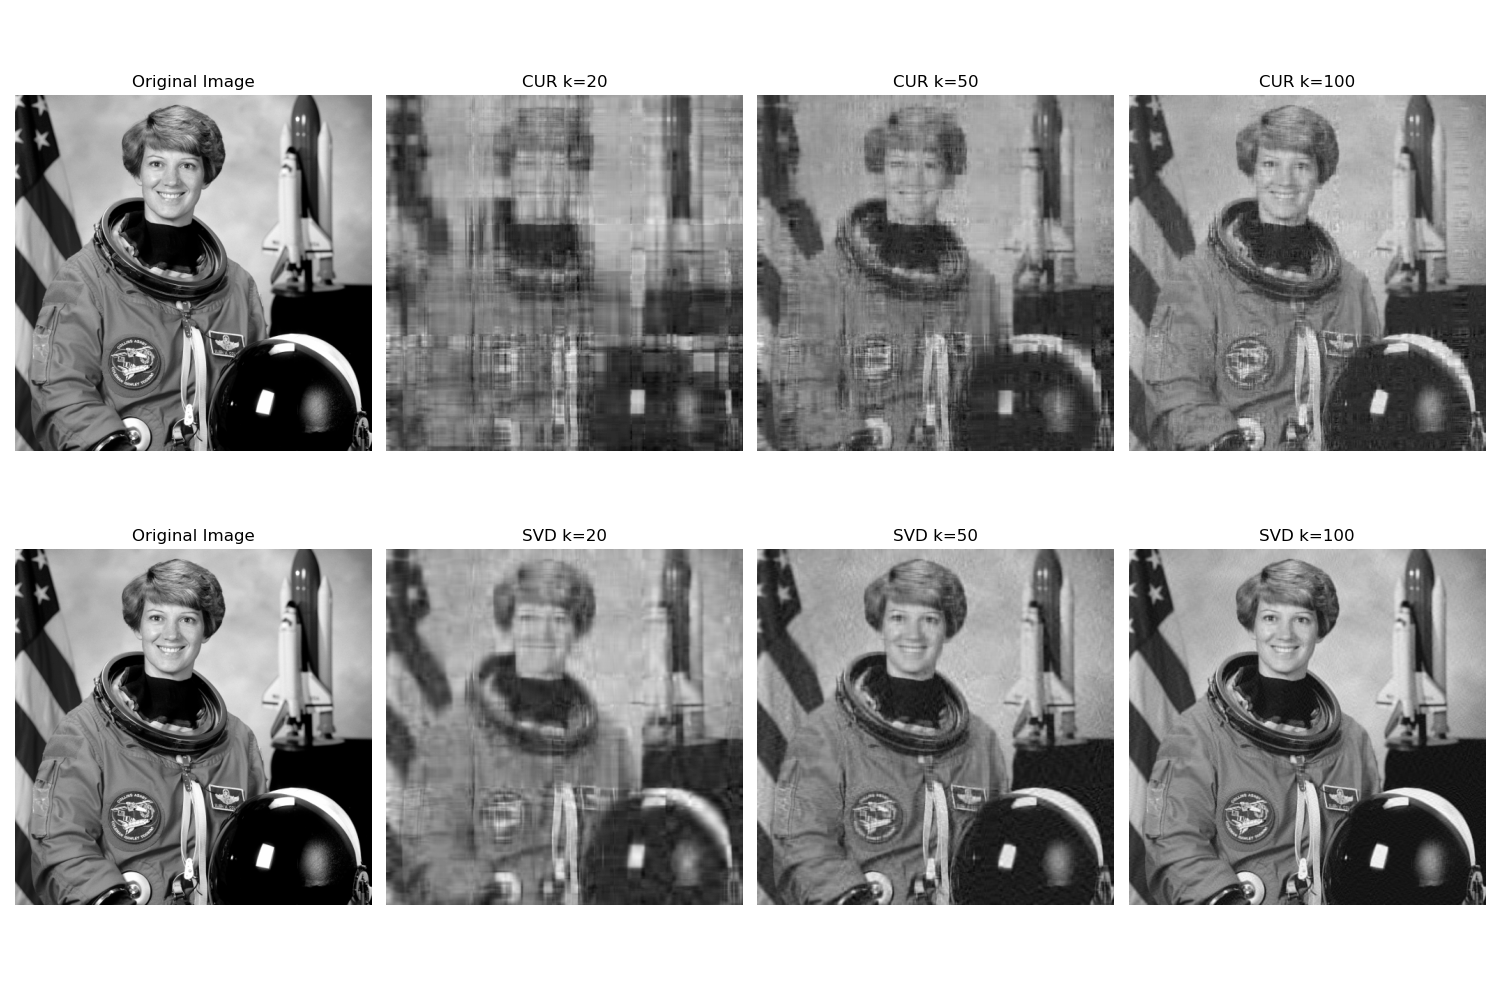
\includegraphics[width=0.8\textwidth]{C:/codestuffs/Numerical-Linear-Algebra/finalproj/imcomp.png}
        \caption{Comparison of the original image with its CUR-compressed version}
        \label{fig:lena_compression}
    \end{figure}
\end{frame}

\begin{frame}{Computational Time Comparison for CUR Compression}
    \begin{figure}
        \centering
        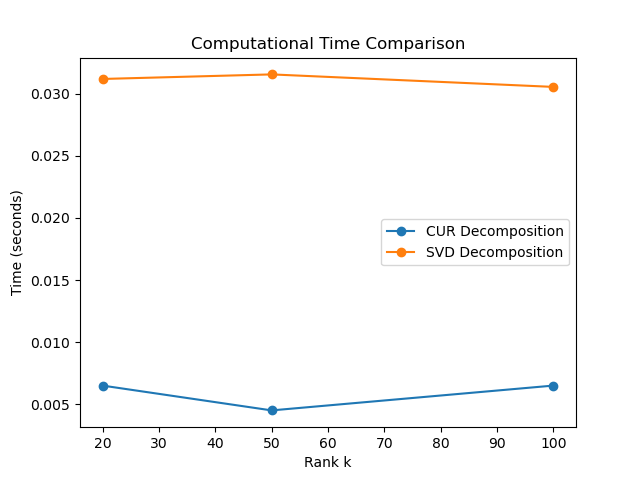
\includegraphics[width=0.8\textwidth]{C:/codestuffs/Numerical-Linear-Algebra/finalproj/imcomptime.png}
        \caption{Graph showing the computational time comparison between CUR and SVD image compression}
        \label{fig:compression_time}
    \end{figure}
\end{frame}

\begin{frame}{Applications in Data Mining and Machine Learning}
    \begin{itemize}
        \item \textbf{Use Cases:}
            \begin{itemize}
                \item CUR is instrumental in systems where the interpretability of decomposed matrices is crucial, such as detailed data analysis and feature selection processes in bioinformatics and text mining.
                \item Enhanced feature selection leads to more robust machine learning models by retaining only the most significant predictors.
            \end{itemize}
    \end{itemize}
\end{frame}

\begin{frame}{Real-world Example: Genomic Data Analysis}
    \frametitle{CUR in Genomic Data Analysis}
    \begin{itemize}
        \item \textbf{Data Matrix Description:}
        \begin{itemize}
            \item Dimensions: 2000 genes (rows) × 14 expression level assays (columns).
            \item Content Variability: Includes genes with different types of transcriptional responses—noise, noisy sine pattern, and noisy exponential pattern.
        \end{itemize}
        \item \textbf{CUR Approach:}
        \begin{itemize}
            \item Selection Based on Leverage Scores: High statistical leverage indicates significant influence on the data's structure.
            \item Interpretability and Insight: Enhances the ability to identify specific genes contributing to observed patterns, improving biological relevance.
        \end{itemize}
    \end{itemize}
    \footnote{\cite{MahoneyDrineas2009}}
\end{frame}

\begin{frame}{Real-world Example: Genomic Data Analysis}
    \begin{itemize}
        \item \textbf{Key Discoveries:}
        \begin{itemize}
            \item Focused Analysis on Influential Genes: Highlights biologically significant patterns, useful for experimental validation.
            \item Direct Link to Biological Processes: Facilitates understanding of gene regulation and responses, crucial for drug discovery.
        \end{itemize}
        \item \textbf{Example Outcomes:}
        \begin{itemize}
            \item Enhanced Data Interpretation: Pinpoints specific gene expression patterns.
            \item Practical Applications: Vital for areas like drug discovery, where specific gene responses to treatments are studied.
        \end{itemize}
    \end{itemize}
    \footnote{\cite{MahoneyDrineas2009}}
\end{frame}



\begin{frame}{Computational Cost Comparison}
            \begin{itemize}
                \item \textbf{CUR Decomposition:} 
                    \begin{itemize}
                        \item CUR decomposition involves selecting a subset of columns and rows from the original matrix, which can be computed efficiently using randomized algorithms such as leverage score sampling.
                        \item The computational cost of CUR is often \(O(SVD(A,k)) = O(mnk)\) \cite{MahoneyDrineas2009}, where \(n\) is the number of rows, \(m\) is the number of columns and \(k\) is the desired rank, making it suitable for real-time processing and big data applications.
                    \end{itemize}
                \item \textbf{Comparison with Other Techniques:}
                    \begin{itemize}
                        \item \textbf{SVD (Singular Value Decomposition):} SVD typically has a computational complexity of \(O(n^2 \cdot m)\) for an \(n \times m\) matrix, making it computationally expensive, especially for large matrices.
                        \item \textbf{PCA (Principal Component Analysis):} PCA's computational complexity is \(O(n^3)\) for computing eigenvalues and eigenvectors of the covariance matrix, which can be high for high-dimensional data.
                    \end{itemize}
            \end{itemize}
\end{frame}




\begin{frame}{CUR vs. PCA: A Comparative Analysis}
    \begin{itemize}
        \item \textbf{Objective Differences:}
            \begin{itemize}
                \item PCA seeks to maximize variance captured by projecting the data onto orthogonal principal components.
                \item CUR selects actual rows and columns, aiming to preserve the matrix structure and interpretability.
            \end{itemize}
        \item \textbf{Performance in Sparse Data:}
            \begin{itemize}
                \item PCA can struggle with sparse data where the variance is not a straightforward indicator of data structure importance.
                \item CUR excels in sparse settings due to its direct selection of influential matrix elements.
            \end{itemize}
        \item \textbf{Use Cases:}
            \begin{itemize}
                \item PCA is preferred in dense datasets and scenarios where dimensionality reduction is crucial.
                \item CUR is advantageous in applications requiring direct interpretation of the original features, such as text analysis and genomic data.
            \end{itemize}
    \end{itemize}
\end{frame}


\begin{frame}{Conclusion}
    \frametitle{Conclusion}
    \begin{itemize}
        \item \textbf{Unique Advantages:}
            \begin{itemize}
                \item \textbf{Interpretability:} CUR allows users to retain actual rows and columns from the original dataset, enhancing the interpretability of results, crucial in fields such as genomics and social sciences.
                \item \textbf{Efficiency:} Particularly effective for large sparse matrices, CUR can be more efficient than traditional SVD, reducing computational load and memory usage.
            \end{itemize}
        \item \textbf{Potential Limitations:}
            \begin{itemize}
                \item \textbf{Dependency on Initial Selection:} The performance of CUR heavily depends on the choice of columns and rows, which can vary significantly with different selection methods.
                \item \textbf{Approximation Quality:} While CUR provides a useful approximation, it might not always achieve the same level of accuracy as the best rank-k approximation provided by SVD, particularly in tightly coupled datasets.
            \end{itemize}
    \end{itemize}
\end{frame}

\begin{frame}{Future Directions}
    \frametitle{Future Research and Applications}
    \begin{itemize}
        \item \textbf{Improving Accuracy and Efficiency:}
            \begin{itemize}
                \item \textbf{Advanced Algorithms:} Research into more sophisticated algorithms for selecting columns and rows could enhance both the accuracy and efficiency of CUR decompositions.
                \item \textbf{Hybrid Approaches:} Combining CUR with other matrix factorizations or machine learning models to improve performance and stability.
            \end{itemize}
        \item \textbf{Emerging Applications:}
            \begin{itemize}
                \item \textbf{Deep Learning:} Exploring the use of CUR in optimizing neural network training by efficiently approximating weight matrices.
                \item \textbf{Network Analysis:} Applying CUR to the study of network flow and connectivity patterns in large-scale networks, potentially improving the understanding of complex systems like internet traffic or social networks.
                \item \textbf{Real-time Data Processing:} Utilizing CUR in real-time data systems, such as streaming data analysis and online learning environments, where quick and efficient data processing is crucial.
            \end{itemize}
    \end{itemize}
\end{frame}

\begin{frame}{Bibliography}
    \frametitle{References}
    \begin{thebibliography}{10} % '10' here indicates the maximum number of entries to be added; increase if more citations are present
        \setbeamertemplate{bibliography item}[text]
        
        \bibitem{MahoneyDrineas2009}
        M. W. Mahoney and P. Drineas,
        \newblock {\em CUR Matrix Decompositions for Improved Data Analysis},
        \newblock 2009.
        \newblock This reference discusses the computational considerations and real-world applications of CUR matrix decomposition, particularly in genomic data analysis.
        
        % Add more \bibitem entries for each additional reference.
    \end{thebibliography}
\end{frame}


\end{document}
